\section{Architecture}\label{sec:architecture}

Although this paper focuses only on scheduling system's core,
the architecture keeps in mind future work on whole infrastructure.
Therefore us the system's architecture based on the idea of cooperating microservices,
where each service has control over specific part of the infrastructure. 

Microservice architecture is an software design architectural style 
that structures an application as a collection of loosely coupled services that 
are organized around system's business capabilities\cite{namiot2014micro} 
and are independently deployable with enabled continuous delivery\cite{balalaie2016microservices}.

\subsection{Architecture scheme}\label{subsec:architecture-scheme}
Following scheme proposes system's core architecture only. 
Implementation itself was developed accordingly 
and used technologies and techniques are described in following sections.

\begin{figure}[ht]
    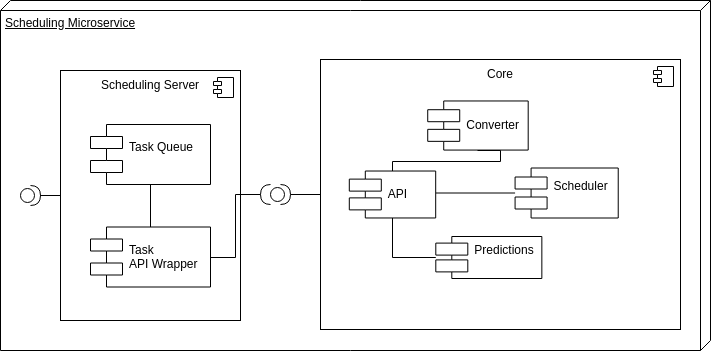
\includegraphics[width=\textwidth]{i_scheduler.png} 
    \centering
    \caption{Microservice architecture with scheduling core}
    \label{fig:scheduling-core-arch}
\end{figure}



\subsubsection{Simulations architecture}\label{subsec:simulations-architecture}
Simulations module is designed as another microservice to simulate future load balancing system's behavior.
It contains something\ldots

\begin{figure}[ht]
    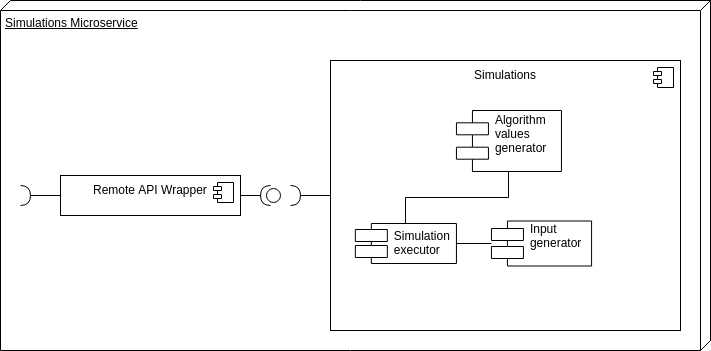
\includegraphics[width=\textwidth]{i_simulations.png}
    \centering
    \caption{Simulations module scheme}
    \label{fig:simulations-arch}
\end{figure}